\begin{sectionbox}[Eager Mode Execution]\nospacing
    \begin{circlelistnosep}
        \item
    \imp{Operation Execution}:\\
    During eager-execution, a \pythoninline{grad_fn} is created for each operation.
    For each input tensor \pythoninline{collect_next_edges} adds an edge to the \pythoninline{grad_fn} of the input tensor and adds the link to \pythoninline{grad_fn.next_functions} array.\\
    For input tensors without a \pythoninline{grad_fn}, \pythoninline{collect_next_edges} links to the special function \pythoninline{AccumulateGrad}.
    \item \imp{Backward}:
    \pythoninline{Autograd} calcualtes the gradients using the rules of \pythoninline{grad_fn} and accumulates results into the \pythoninline{grad} fields of the tensors.
    \end{circlelistnosep}
    \begin{figure}[H]
        \centering
        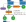
\includegraphics[width=1.0\textwidth]{pytorch_submodule/src/the_framework/basics/automatic_differentiation/autograd/figures/graph.pdf}
    \end{figure}
\end{sectionbox}
\begin{defnbox}\nospacing
    \begin{defn}[\tcblack{\pythoninline{grad_fn}}]\leavevmode\\
        Is the main function object that:
        \begin{itemizenosep}
            \item represents operations and their derivatives
            \item represents nodes in the computational graphs and links to the previous functions that created the current tensor using \pythoninline{grad_fn.next_functions}.
        \end{itemizenosep}
    \end{defn}
\end{defnbox}
\begin{defnbox}\nospacing
    \begin{defn}[\tcblack{\pythoninline{grad_fn.next_functions}}]\leavevmode\\
        Is an array of \pythoninline{grad_fn, pos} tuples, where
        \begin{itemizenosep}
            \item the \pythoninline{grad_fn} points to the previous (older for in-forward) operation
            \item \pythoninline{pos} represents the position of the current tensor in the \pythoninline{grad_fn} of the previous input tensor
        \end{itemizenosep}
    \end{defn}
\end{defnbox}
\begin{notebox}[Notes]\nospacing
    \begin{itemizenosep}
        \item Position is important for the backward pass and functions such as \pythoninline{unbind} which needs to know during automatic differention, which tensor is which: \pythoninline{b, c, a = a.unbind()}
        \item Non leaf gradients are not calculated as the can be calculated implicitly
    \end{itemizenosep}
\end{notebox}
%%% Local Variables:
%%% mode: latex
%%% TeX-command-extra-options: "-shell-escape"
%%% TeX-master: "../../../../../../formulary"
%%% End:
